\chapter{The cloud computing setting}\label{chap:cloudcomputing}


\section{Containers and virtual machines: a short introduction}\label{sec:chpt1-containers}


% Virtual machines, which emerged in the late 1990s and early 2000s, represented
% a significant advancement in computing. By allowing multiple operating systems
% to run concurrently on a single physical machine, VMs brought about
% unprecedented flexibility and efficiency in resource utilization. The
% \textit{hypervisor} facilitates this capability being a crucial piece of
% software that abstracts the underlying physical hardware. There are two main
% types of hypervisors: Type 1 hypervisors, also known as bare-metal hypervisors,
% run directly on the physical hardware. Type 2 hypervisors, on the other hand,
% run on top of an existing operating system \cite{rodriguezharo-2012}. A
% schematic representation of the two types of hypervisors can be seen in Figure
% \ref{fig:VM-vs-Container}. Virtual machines operate by virtualizing all hardware
% resources, creating isolated environments where each VM has its own operating
% system and applications. This architecture ensures strong isolation and security
% between VMs but comes at the cost of efficiency. Each VM needs to run a
% full-fledged operating system, leading to substantial overhead in memory and CPU
% usage. Despite these drawbacks, VMs have been the backbone of data centers and
% cloud infrastructure for years, providing reliable and secure environments for
% diverse applications.

Virtual machines were developed starting in the late 1990s and early 2000s.
Their appearance represented a significant technological advancement in
computing, allowing multiple operating systems to run concurrently on a single
physical machine, sharing its resources without interfering. VMs brought about
unprecedented flexibility, security, and efficiency in resource utilization. The
critical piece of software that made this possible by abstracting the physical
hardware is called \textit{hypervisor}. There are two main types of hypervisors:
Type 1 hypervisors, also known as bare-metal hypervisors, run directly on the
physical hardware. Type 2 hypervisors, on the other hand, run on top of an
existing operating system \cite{rodriguezharo-2012}. A schematic representation
of where the two types of hypervisors fit in a virtualization stack is shown in
Figure \ref{fig:VM-vs-Container}. 

% Virtual machines operate by virtualizing all hardware resources, creating
% isolated environments where each VM has its operating system and applications.
% This architecture ensures strong isolation and security between VMs but comes at
% the cost of efficiency. Each VM needs to run a full-fledged operating system,
% leading to substantial overhead in memory and CPU usage. Despite these
% drawbacks, VMs have been the backbone of data centers and cloud infrastructure
% for years, providing reliable and secure environments for diverse applications.
% It is axiomatic that containers have dethroned virtual machines (VMs) as the
% core technology for cloud computing. This shift is not just a passing trend but
% a fundamental change in how cloud infrastructure is conceived and managed.
% Virtually all scientific literature agrees with this statement, including
% sources like \cite{Casalicchio2020TheSI, Bentaleb2021,
% zhang2018comparativestudycontainersvirtual}. These sources highlight the
% substantial advantages of containers over traditional VMs, cementing their
% status as the de facto standard in modern cloud environments. To understand why
% containerization technologies have become so dominant, we must first examine the
% technological landscape that preceded them.

Virtual machines operate by virtualizing all hardware resources, creating
isolated environments where each VM has its operating system and applications.
This architecture ensures strong isolation and security between VMs but comes at
the cost of efficiency. A VM must run a full-fledged operating system, leading
to substantial overhead in memory and CPU usage. Despite these drawbacks, VMs
have been the backbone of data centers and cloud infrastructure for years,
providing reliable and secure environments for diverse applications. Containers
then appeared to overcome many VMs's limitations and performance bottlenecks.
Thanks to the advantages they brought, they soon became the core technology for
cloud computing. This shift has not been a passing trend but a fundamental
change in how cloud infrastructure is conceived and
managed\cite{Casalicchio2020TheSI, Bentaleb2021,
zhang2018comparativestudycontainersvirtual}. The substantial advantages of
containers over traditional VMs made them the de facto standard in modern cloud
environments. To understand why containerization technologies have become so
dominant, we must review their technical differences from those of VMs.

% Containers are lightweight, portable units that
% bundle an application and its dependencies into a single package.
% Unlike VMs, containers do not require a separate operating system for each
% instance. Instead, they share the host operating system's kernel, drastically
% reducing overhead and allowing for a greater density of applications on a single
% physical machine (see Figure \ref{fig:VM-vs-Container}).
% Under the hood, containers are built on top of the host operating system's
% kernel, which provides the necessary system calls and resources for running
% applications. When a container is started, it runs as a process on the host
% machine, isolated from other containers and the host system.
% Containers achieve their isolation and efficiency through two key technologies:
% \textit{namespaces}, control groups (\textit{cgroups}), and
% \textit{capabilities}.

% Namespaces ensure that each container has its own isolated view of system
% resources such as process trees, network stacks, and file systems. This
% isolation is fundamental to ensuring that containers do not interfere with each
% other, providing a secure environment for each application.
% Cgroups are responsible for limiting and prioritizing resource usage such as
% CPU, memory, and I/O for each container. By managing resources at this granular
% level, cgroups ensure that each container operates efficiently without impacting
% the performance of other containers on the same host.
% Capabilities are a way to control a process's access to system resources. By
% granting or restricting capabilities, containers can be fine-tuned to have the
% necessary permissions to perform their tasks without compromising security
% \cite{kerris2021}.

Containers are lightweight, portable units that bundle an application and its
dependencies into a single package. Unlike VMs, containers do not require a
separate operating system for each instance. Instead, they share the host
operating system's kernel, drastically reducing overhead and allowing for a
greater density of applications on a single physical machine. On the right side
of fig.~\ref{fig:VM-vs-Container} is reported a schematic comparison between the
VM's software stack and a container's software stack. Under the hood, containers
are built on top of the host operating system's kernel, which provides the
necessary system calls and resources for running applications. When a container
is started, it runs as a process on the host machine, isolated from other
containers and the host system. Containers achieve their isolation and
efficiency through two key technologies: \textit{namespaces}, control groups
(\textit{cgroups}), and \textit{capabilities}. Namespaces ensure that each
container has its own isolated view of system resources such as process trees,
network stacks, and file systems. This isolation is fundamental to ensuring that
containers do not interfere with each other, providing a secure environment for
each application. Cgroups are responsible for limiting and prioritizing resource
usage such as CPU, memory, and I/O for each container. By managing resources at
this granular level, cgroups ensure that each container operates efficiently
without impacting the performance of other containers on the same host.
Capabilities are a way to control a process's access to system resources. By
granting or restricting capabilities, containers can be fine-tuned to have the
necessary permissions to perform their tasks without compromising security
\cite{kerris2021}.
% TODO we should add a reference for namespace (kerrisk_2013) and a reference for cgroup (like
% Ovens_2020)

The container architecture is built around bundling an application with all its
dependencies into a single, portable unit. This unit can run consistently across
various environments, from development to production.
In order to make the fruition of the following chapters more accessible, it is
necessary to briefly summarize some of the key components usually cited in this
context that sometimes can be confused \cite{walsh2022, huawei2023}:

\begin{itemize}
  \itemsep0em
  \item \textit{Container engine}: is the software responsible for running
    containers. It provides the runtime environment in which containers execute
    and manages the lifecycle of these containers, including their creation,
    start, stop, and removal. Popular container engines include Docker, Podman,
    containerd, and CRI-O. The container engine abstracts the underlying
    operating system, enabling the containers to run consistently across various
    environments without concern for platform-specific dependencies.
  \item \textit{Container runtime}: is the software responsible for executing
    containers. It is the component that interacts directly with the host
    operating system's kernel to create and manage containers. The container
    runtime is typically integrated with the container engine, providing the
    low-level functionality needed to run containers.
  \item \textit{Image}: is a lightweight, stand-alone, and executable software
    package that includes everything needed to run a piece of software. This
    includes the code, runtime, libraries, environment variables, and
    configuration files. Images are immutable, meaning once created, they do not
    change. They serve as a blueprint for creating containers, ensuring that the
    application runs the same regardless of where the container is deployed.
  \item \textit{Container}: is a runtime instance of a container image. It is
    ephemeral, meaning it can be created, started, stopped, and removed quickly
    and easily.
  \item \textit{Orchestrator}: An orchestrator is a tool that automates the
    deployment. More detail will be provided in the dedicated paragraph
    \ref{sec:chpt1-orchestrator}.
\end{itemize}


\begin{figure}[h]
    \centering
    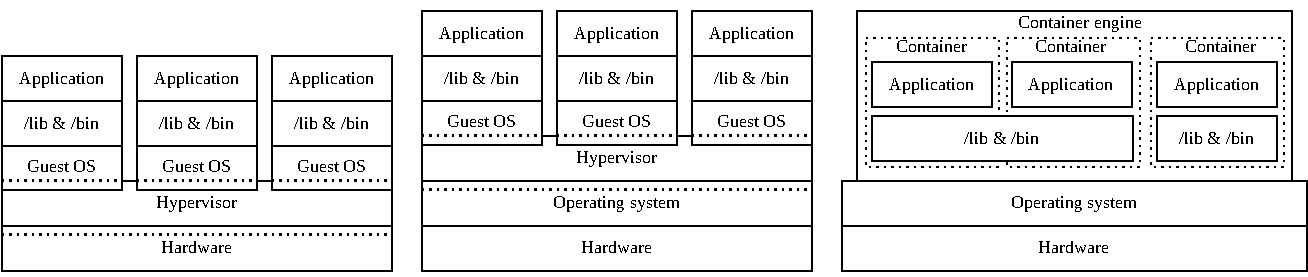
\includegraphics[width=\textwidth]{img/chpt1/VM-vs-Container}
    \caption{From left to right: schematic representation of how a VM with type 1 hypervisor (left), type 2 hypervisor (center), and a container (right) works. In the first two cases, the user application (on top) runs inside a fully-fledged operative system that runs its kernel in a completely isolated environment. The type one hypervisor can be realized with the Linux kernel using the Kernel-based Virtual Machine (KVM)  module. In this case, each virtual processor issues instructions directly to the physical processor, limiting overhead. In the type two hypervisor, instructions are not directly fed to the processor but are pre-processed by other software that, for example, might be responsible for instruction emulations (if running from different architectures). This second type of hypervisor can be realized again with a Linux kernel and a plain Quick Emulator (QEMU). Such a solution also gives the advantage of emulating hardware peripherals not present in the actual host. The QEMU/KVM stack is commonly deployed to obtain the best of both worlds: hardware emulation and almost native CPU performance. The latter case on the right is the container case. Here, the user application runs in an isolated environment (the container) controlled by the container engine. In this case, however, the container shares the main OS, the kernel, and the hardware with all other containers. The user application is for the main OS, a process in its own right with a valid process identification number that can not perform any action outside the environment.}
    \label{fig:VM-vs-Container}
\end{figure}


\subsection{Portability}\label{subsec:chpt1-portability}

% In the last decades, the scientific community has encountered the issue commonly
% referred to as "dependency hell." This term describes the challenges associated
% with reproducing scientific experiment results across different machines or
% environments. The problem arises due to the reliance of scientific software on
% various libraries, frameworks, and other components. When these dependencies are
% not adequately managed, compatibility issues, version conflicts, and other
% problems can prevent the software from functioning correctly on different
% systems. This "dependency hell" presents a significant obstacle to scientific
% progress, as it impedes the reproducibility of research results and complicates
% the sharing and collaboration on scientific code. Notably, both technologies
% mentioned above were developed as solutions to this problem.
% When examining the range of solutions adopted by the scientific community over
% the years (as summarized in Figure \ref{fig:solspectrum}), it becomes evident
% why the trade-off containers offer is often considered the most appealing
% \cite{sarusso}.

One of the leitmotifs of software management that has not left out the
scientific community is the issue commonly known as "dependency hell." This
term,  in science, represents the challenges the researcher must overcome to
reproduce scientific experiment results across different machines or
environments. The problem arises due to the reliance of scientific software on
various libraries, frameworks, and other components that change between
environments. When these dependencies are not adequately managed, compatibility
issues, version conflicts, and other problems can prevent the software from
functioning correctly on different systems. This "dependency hell" presents a
significant obstacle to scientific progress, as it impedes the reproducibility
of research results and complicates the sharing and collaboration on scientific
code. Notably, both technologies mentioned in the previous section were
developed to solve this problem. When examining the range of solutions adopted
by the scientific community over the years (as summarized in Figure
\ref{fig:solspectrum}), it becomes evident why the trade-off containers offer is
often considered the most appealing \cite{sarusso}.

% Such libraries often come with the convenience that they are incompatible with
% one another and are tangled together in a way that does not allow for simple
% replacements.

% Starting from the left side of the spectrum (as referenced in Figure
% \ref{fig:solspectrum}), reliance on a well-written requirements file,
% accompanied by suitable documentation from the software developer, represents
% the most straightforward solution. However, this approach is also highly
% error-prone. Additionally, it requires users to manually install all
% dependencies listed in the requirements file, which may not always be possible
% due to conflicts between different versions of the same library or framework or
% if the user lacks the necessary permissions.

Figure \ref{fig:solspectrum}  qualitative summarizes how different approaches in
software distribution reflect on critical metrics that a researcher should
consider when publishing his code. Starting from the most appealing in an HPC
context on the left side of the spectrum, we have the typical compilation that
relies on a well-written requirements file and suitable documentation from the
software developer. This approach represents the most straightforward solution
but is also highly error-prone. Additionally, it requires users to manually
install all dependencies listed in the requirements file, which may not always
be possible due to conflicts between different versions of the same library or
framework or if the user lacks the necessary permissions.

% Creating statically linked binaries offers a more convenient solution with
% minimal effort required from the user. In this case, all dependencies are
% included within the binary itself, eliminating the need for users to install
% them separately. Although this approach is practical (with the only limitations
% being the operating system and processor architecture), it has certain drawbacks
% that have limited its widespread adoption. Specifically, this method cannot be
% applied to interpreted languages, including popular ones in scientific computing
% such as Python, R, and Julia.

Creating statically linked binaries offers a more convenient solution with
minimal user effort. In this case, all dependencies are included within the
binary, eliminating the need for users to install them separately. Although this
approach is practical (with the only limitations being the operating system and
processor architecture), it has certain drawbacks that have limited its
widespread adoption. Specifically, this method cannot be applied to interpreted
languages (including popular ones in scientific computing such as Python, R, and
Julia); it tends to produce large files, and the produced binary needs to be
targeted to a specific architecture.

% On the opposite end of the spectrum, virtual machines (VMs) are worth noting.
% The ability to perform hardware emulation, which allows software to run in an
% environment completely isolated from the host machine, represents a technically
% effective solution to the dependency hell problem. However, this approach also
% incurs significant overhead. Consequently, it is seldom mentioned except in
% recent years, as the x86-64 processor architecture has become the de facto
% standard. For typical VMs (without emulation), portability across different
% operating systems is maintained, and once an image is created, it can be easily
% shared and run on different machines. The primary drawback, as discussed in
% paragraph \ref{sec:chpt1-orchestrator} of this chapter, is the overhead in terms
% of memory and CPU usage, which can be substantial when running multiple VMs on
% the same host machine. Additionally, the startup time for a VM is generally much
% longer than that of a container, making VMs less suitable for short-lived tasks
% or applications that require rapid scaling.

% TODO review this paragraph, it is not very clear
On the opposite end of the spectrum, there are VMs. In this case, inside the VM,
we have a completely portable software stack, and we can perform hardware
emulation, which allows the software to run in an environment different from the
host machine and mimic the development one. This solution is technically very
effective against the dependency hell problem. However, this approach also
incurs significant overhead. The possibility of simulating hardware has seldom
been mentioned in the last decade as the x86-64 processor architecture has
become the de facto standard. Thanks to RISC-V and Advanced RISC Machines (ARM),
it has risen again in popularity. For typical VMs (without emulation),
portability across different host operating systems is always working, and once
an image is created, it can be easily shared and run on different machines.
Stressing the drawbacks, as discussed in paragraph \ref{sec:chpt1-orchestrator}
of this chapter, the overhead of memory and CPU usage can be substantial when
running multiple VMs on the same host machine. Additionally, the startup time
for a VM is generally much longer than that of a container, making VMs less
suitable for short-lived tasks or applications that require rapid scaling.

\begin{figure}[h]
    \centering
    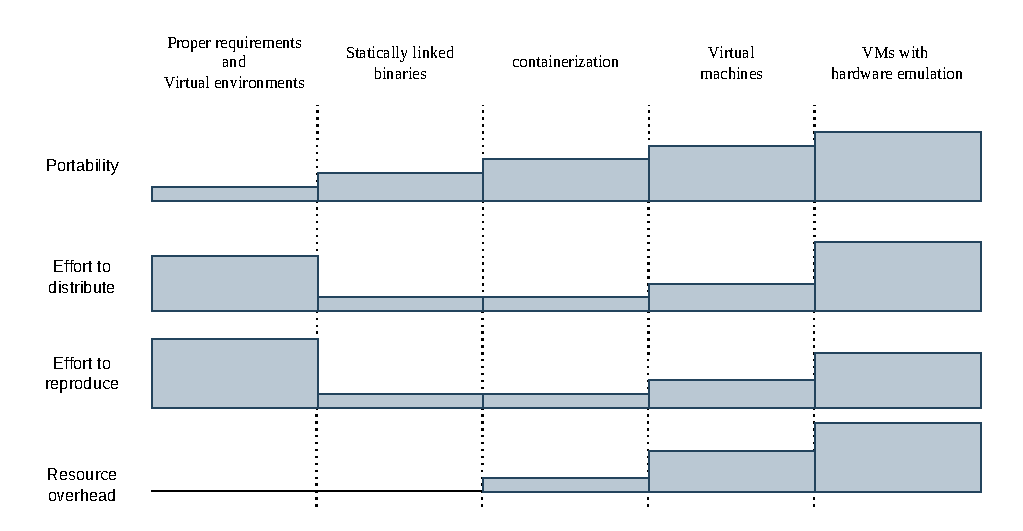
\includegraphics[width=\textwidth]{img/chpt1/solutions-spectrum}
    \caption{Qualitative overview of the main advantages and disadvantages of
      various packaging solutions to distribute software vs critical metrics for
      the ``dependency hell'' problem to consider when publishing a code}
    \label{fig:solspectrum}
\end{figure}


\subsection{Container performance}

As previously mentioned, containers offer greater flexibility and portability
and represent a more efficient solution for extracting maximum performance from
the underlying hardware.
It is now essential to provide a detailed analysis of
the performance aspects of containers, as this topic has garnered significant
attention in the specialized literature.
The performance of containers has been extensively studied, with particular
emphasis on how they compare to traditional virtualization techniques, such as
those utilizing hypervisors.
Noteworthy contributions in this area include the works of Sharma et al.
\cite{Sharma2016}, Deochake et al. \cite{deochake2023}, and Li et al.
\cite{Li2023}.

These studies consistently demonstrate that the virtualization process employed
by hypervisors introduces considerable performance overhead.
This overhead arises due to hypervisors needing to emulate hardware and manage
virtual machines, thereby adding layers of abstraction between the application
and the physical resources.
The added complexity leads to slower I/O operations, increased latency, and
reduced throughput, ultimately resulting in performance degradation.
In contrast, containerization, which operates at the operating system level,
circumvents much of this overhead by sharing the host OS kernel.
Containers provide isolated environments for applications while allowing direct
access to underlying hardware resources. Consequently, containerized
applications' performance closely approximates native, bare-metal solutions,
with differences being negligible in most cases.
This efficiency renders containers particularly attractive for high-performance
computing and other resource-intensive applications, where minimizing overhead
is critical.

Another significant study by Mohammadi et al. \cite{Mohammadi2018} explores the
feasibility of utilizing cloud computing environments to perform workloads
typically associated with high-performance computing (HPC) facilities.
Notably, the widely recognized LINPACK benchmark, used to measure the
performance of supercomputers, was executed on a cloud infrastructure with
highly satisfactory results.

It is important to note that all the studies mentioned earlier focus on
assessing the computational performance of containers. While this is a crucial
factor, there are other considerations when evaluating the suitability of cloud
infrastructure as a candidate for distributed scientific computing.
As will be discussed in subsequent chapters (see Chapters \ref{chpt:cni} and
\ref{chpt:osu}), network and I/O performance are also critical aspects that
require careful evaluation. These two factors have become increasingly
significant and are now recognized as primary bottlenecks in modern
infrastructure.

\section{Orchestrator: using a container-based setting in the modern era}\label{sec:chpt1-orchestrator}

%% 5 pagine

%% Quali sono le belle features che ci da un orchestrator?
%%   • Scalability
%%   • Availability
%%   • Load balancing
%%   • Fault tolerance
%%   • RBAC (Role Based Access Control)


With the advent of containerization technologies and the rise of cloud
computing, the need for efficient management of containers has become
increasingly apparent.
This requirement has given rise to a new class of tools known as container
orchestrators. These orchestrators play a crucial role in automating
containerized applications' deployment, scaling, and management, thereby
simplifying the complex container management processes \cite{Rodriguez2018}.
They make deploying, operating, and maintaining intricate applications in
dynamic cloud environments easier.

As is often the case in the open-source ecosystem, numerous solutions have been
developed to address this need.
Some of the most notable orchestrators include Kubernetes
\cite{bookofkubernetes}, OpenStack \cite{Lima2017}, and Docker Swarm
\cite{Singh2023}.
Each of these orchestrators has been designed to meet the diverse requirements
of cloud infrastructure management, offering unique functionalities that cater
to different use cases.
Before delving into the specifics of the orchestrator employed in this study, it
is essential to examine the key features orchestrators typically provide, making
them indispensable tools for managing containerized applications.

\subsection{Scalability}

One of the primary benefits of using an orchestrator is its ability to scale
applications quickly and efficiently.
Orchestrators allow to define of scaling policies that automatically adjust the
number of containers running in response to changes in demand.
This feature is particularly advantageous for applications with variable
workloads, as it ensures that resources are allocated appropriately to meet
demand without over-provisioning.
By dynamically scaling containers, orchestrators help optimize resource
utilization and reduce operational costs, thereby enhancing the overall
efficiency of cloud infrastructure management.
The scaling capabilities of orchestrators can be broadly categorized into two
main types: vertical scaling and horizontal scaling.

\textit{Vertical scaling} refers to increasing the resources available to a single
container, such as CPU, memory, or disk space.
This approach is advantageous when an application requires more resources than
initially allocated.
The user can perform vertical scaling manually or automatically with the
orchestrator based on predefined policies.
Notably, unlike vertical scaling in traditional virtual machines (VMs), which
often requires stopping and restarting the instance, vertical scaling in
containers can typically be accomplished without interrupting the running
instance, thus ensuring continuous availability and demonstrating once again
some of the benefits of containerization.

\textit{Horizontal scaling}, on the other hand, involves adding more instances of a
container to distribute the workload across multiple containers.
This method is particularly effective for applications that handle parallel and
independent tasks, as it allows the workload to be spread across several
instances, thereby improving performance and resilience.
Horizontal scaling also plays a crucial role in ensuring high availability and
fault tolerance, as it enables the system to maintain functionality even in the
event of individual container failures (see Section
\ref{subsec:chpt1-availability} for a more detailed discussion).

Both vertical and horizontal scaling are autonomously managed by the
orchestrator, which continuously monitors the application's performance and
makes scaling decisions based on policies defined by the cluster administrator.
This level of automation ensures that the application can respond quickly and
efficiently to fluctuations in demand, providing a seamless experience for
end-users.
While CPU and memory usage are the most common metrics used to guide scaling
decisions, orchestrators are also capable of considering other factors such as
network traffic, disk I/O, or custom application-specific metrics, allowing for
a more tailored and responsive scaling strategy \cite{Qu2016}.

\subsection{Availability and self-healing}\label{subsec:chpt1-availability}

Ensuring high availability and fault tolerance is a cornerstone of managing any
production system, and this obviously applies to cloud environments as well.
Orchestrators are pivotal in maintaining application availability and enabling
systems to recover from failures autonomously.

A fundamental feature that orchestrators provide is \textit{self-healing}.
Self-healing refers to the orchestrator's capability to automatically detect,
respond to, and recover from system failures without human intervention.
For instance, when a container or node fails, the orchestrator can automatically
restart the failed container on a healthy node, thereby maintaining the
application's availability and responsiveness.
This ability is especially critical in distributed systems, where failures are
common and can occur unpredictably.
By automating recovery processes, orchestrators significantly reduce downtime,
ensuring continuous operation despite disruptions.
Two fundamental mechanisms associated with self-healing are \textit{liveness
  probes} and \textit{readiness probes}. These probes are integral to monitoring
and managing the health of containers:

\begin{itemize}
  \itemsep0em
   \item \textit{Liveness Probes}: are a proactive measure to ensure the
     container's health.
     They regularly check the container's status, and if a probe fails, the
     orchestrator interprets this as a sign of a faulty container.
     As a result, the orchestrator may terminate and restart the container to
     restore it to a healthy state. This proactive approach prevents prolonged
     service degradation or outages, providing a sense of reassurance about the
     system's robustness.
    \item \textit{Readiness Probes}: determine whether a container is ready to
      handle incoming traffic.
      By assessing the container's readiness to serve requests, they ensure that
      only fully operational and correctly initialized containers receive requests.
      This user-centric approach enhances the overall user experience and
      reliability, making the audience feel the system is designed to meet their
      needs.
\end{itemize}

In addition to liveness and readiness probes, orchestrators utilize
\textit{health checks} to monitor the status of containers and nodes.
Health checks are systematic assessments ensuring containers and nodes function
within acceptable parameters.
By conducting regular health checks, orchestrators can detect potential issues
early and initiate corrective actions to prevent system downtime. This proactive
monitoring is essential for maintaining the integrity and performance of
large-scale distributed systems.

Beyond self-healing, orchestrators provide robust mechanisms for ensuring high
availability, one of which is \textit{replication and redundancy}.
Replication involves running multiple instances of an application across
different nodes.
This approach ensures the application remains available even if one or more
instances fail.
By distributing the workload across multiple instances, redundancy mitigates the
risk of a single point of failure and enhances the system's overall resilience
and fault tolerance.
By integrating self-healing capabilities with replication, redundancy, and
health checks, orchestrators offer a comprehensive framework for achieving high
availability and fault tolerance \cite{Brendan2016}.
This framework is essential for modern cloud-based systems, where the demand for
continuous availability and resilience against failures is paramount.


\subsection{Load balancing and fault tolerance}\label{subsec:chpt1-load balancing}

The next great feature that orchestrators provide is load balancing and fault
tolerance.
These two features are critical components in modern cloud infrastructure,
working hand in hand to ensure optimal performance, high availability, and
resilience against failures.

\textit{Load balancing} refers to distributing incoming network traffic across
multiple servers or containers.
This distribution helps to optimize resource utilization, maximize throughput,
minimize response time, and avoid overload of any single resource.
In the context of container orchestration, load balancing is typically
implemented at two levels:
\textit{Service-level load balancing}: This occurs within a cluster,
distributing traffic among multiple instances of the same service or
application.
The orchestrator ensures that incoming requests are evenly distributed across
all available instances, preventing any single container from becoming a
bottleneck.
The second level is \textit{Cluster-level load balancing}: This involves
distributing traffic across multiple nodes in a cluster.
It ensures the workload is balanced across the entire infrastructure, preventing
individual nodes from overloading.
Orchestrators typically employ sophisticated algorithms for load balancing, such
for example \cite{Shafiq2022}:
\begin{itemize}
  \itemsep0em
    \item \textit{Round-robin}: A straightforward method that distributes
      requests sequentially across available instances.
      This approach is simple and effective when the instances are relatively
      uniform regarding capacity and performance.
    \item \textit{Least Connections}: Directs traffic to the instance currently
      handling the fewest connections, ensuring that cases with lighter loads
      are utilized first.
      This strategy is advantageous when instances have varying capacities, or
      the workload is unevenly distributed over time.
    \item \textit{Weighted Load Balancing}: Assign weights to instances based on
      capacity or performance characteristics. Instances with higher weights
      receive more traffic, enabling a more sophisticated and resource-aware
      load distribution.
    \end{itemize}

\textit{Fault tolerance}, on the other hand, is the ability of a system to
continue operating correctly in the event of the failure of some of its
components.
In containerized environments, fault tolerance is closely tied to the concepts
of high availability and self-healing discussed earlier.
Orchestrators implement fault tolerance through several mechanisms:
\begin{itemize}
  \itemsep0em
  \item \textit{Replication}: By maintaining multiple instances of each service
    across different nodes, the system can continue to function even if some
    instances fail.
  \item \textit{State management}: Orchestrators often provide mechanisms for
    managing stateful applications, ensuring that critical data persists and can
    be recovered in case of failures.
  \item \textit{Automatic rescheduling}: When a node fails, the orchestrator
    automatically reschedules the affected containers on healthy nodes,
    minimizing downtime.
  \item \textit{Rolling updates}: This feature allows for updating applications
    without downtime by gradually replacing old instances with new ones,
    reducing the risk of system-wide failures during updates.
\end{itemize}

The synergy between load balancing and fault tolerance is particularly evident
in how orchestrators handle node failures.
When a node becomes unresponsive, the load balancer system quickly redirects traffic
from the failed node to healthy ones.
Simultaneously, the orchestrator's fault tolerance mechanisms kick in,
rescheduling the affected containers on other available nodes. This coordinated
response ensures minimal disruption to the overall system.
By effectively implementing load balancing and fault tolerance, orchestrators
significantly enhance the reliability and performance of containerized
applications.

\subsection{Role-based access control (RBAC)}\label{subsec:chpt1-rbac}

In any infrastructure meant to be used by several users, having granular
control over permissions and authorization each user has is crucial; from this
point of view, a cloud infrastructure does not make any exception.
The typical way to do that in a cloud-based environment is relying on RBAC.
\textit{Role-based access control} is a security paradigm that restricts
access to system resources based on the roles assigned to individual users or
services rather than their individual identities.
This approach simplifies the management of access permissions in large,
distributed environments and enhances security by ensuring that users and
services can only perform actions they are explicitly permitted to.

In particular in Kubernetes, the orchestrator that is going to be used in this
work (see section \ref{sec:chpt1-kubernetes}) RBAC is a core feature that
involves thee main components: \textit{Roles}, \textit{Role Bindings}, and
\textit{Subjects} \cite{kdoc-rbac}:

\begin{itemize}
  \itemsep0em
   \item \textit{Roles}: define a set of permissions, specifying what actions
     are allowed on specific resources within the orchestration environment.
     These actions, also known as \textit{verbs}, may include operations like
     \textit{get},  \textit{create}, \textit{update}, and \textit{delete}.
     Roles are abstract entities not directly assigned to users; instead, they
     encapsulate the permissions that can be granted to a user or service.
   \item \textit{Role Bindings}: are associations that link a \textit{subject}
     \textit{Role}.
     Role bindings effectively grant the permissions defined in a role to the
     specified subject within a particular namespace or across the entire
     cluster, depending on the binding scope.
     There are two types of role bindings: \textit{RoleBindings}, which apply to
     a specific namespace, and \textit{ClusterRoleBindings}, which apply to the
     entire cluster.
   \item \textit{Subjects}: represent the entities (users, groups, or service
     accounts) granted access to the system resources based on their associated
     role bindings. Each subject can be associated with one or more roles,
     allowing for fine-grained control over what each user or service can do
     within the orchestration environment.
\end{itemize}

\section{Kubernetes: the orchestrator of choice}\label{sec:chpt1-kubernetes}

\subsection{Why Kubernetes?}

As previously stated, in the years, many container orchestrators have been
deployed and proposed.
Among the most popular ones, we can mention \textit{Docker Swarm},
\textit{Apache Mesos}, \textit{OpenStack}, and \textit{Kubernetes}.
In the preliminary steps of this work, Docker Swarm, OpenStack, and Kubernetes
were considered possible choices.

Docker swarm \cite{Singh2023} is a container orchestrator developed by Docker
that is integrated into the Docker Engine (at least for the Linux version).
It is designed to be simple to use and easy to set up, but it lacks some of the
advanced features provided by other orchestrators.
In particular, the most severe limitation, which alone was enough to discard it,
is that, at least at the moment this thesis is composed (2024), it does not
support multi-node installation. Since the stated aim is to reproduce HPC in a
cloud-fashion environment, performing distributed computation to guarantee
horizontal scaling is necessary.

The second option, OpenStack, is a mature project initially developed by the
OpenStack Foundation, which is now part of the Open Infrastructure Foundation.
It is a cloud computing platform that provides various services for building and
managing public and private clouds.
One peculiarity distinguishing OpenStack from other alternatives is that it is
more oriented to the infrastructure as a Service (IaaS) model, allowing, for
example, the orchestration of both container and VMs.
In addition to having as its primary focus a use case different from the
objectives of this thesis, the main limitation that led to the exclusion of
OpenStack is the amount of resources needed to deploy such a complex system.

According to the documentation of the current last version (4.16)
\cite{openstakinstallationdoc}, the minimum requirements for deployment are
three nodes that act as a control plane, each of them with an amount of
resources close to one of the nodes of the available infrastructure in the ORFEO
cluster\footnote{In particular the main limitation is the number of cores for
  each node: 22, the RAM: 88GB and the storage requirements 275GB}.
Kubernetes, on the other side, has a much lower footprint and can be deployed
even in a single node with a limited amount of resources\footnote{2-cores CPUs
  and 2Gi of RAM.} \cite{kdoc-installation}, making it more appetite for the
actual infrastructure that was available; see section \ref{sec:measurements} for
more details.

To be fair, the choice of relying on Kubernetes to carry on this work is not
only the consequence of eliminating all the possible alternatives.
The following lines are meant to be a way to (try to) summarize all the nice and
appealing characteristics that make Kubernetes a valuable choice for this work.


\begin{itemize}
  \itemsep0em
  \item \textit{Portability}: Since an entire section
    (\ref{subsec:chpt1-portability}) arguing about the importance of
    portability has been written, it is clear that choosing an orchestrator
    system that takes care of this aspect is a must.
    Technically speaking in fact, \textit{"Kubernetes"} is an API that can be
    implemented by any providers. What makes portable Kubernetes is the fact
    that all the most popular cloud providers (AWS, Azure, Google) have
    implemented the Kubernetes API, making it possible to move workloads between
    different providers without any modification.
  \item \textit{Popularity}: Since its first release in 2014, Kubernetes has
     grant more and more popularity up to becoming the de-facto standard in a great
     variety of cloud contexts.
     This popularity guarantee also the presence of a very active community that,
     like in all valid open source projects, can be a valid support to solve
     possible issues.

   \item \textit{Declarative configuration}: Kubernetes requires a declarative
     approach to configuration, meaning that the user does not need to specify
     how to get a certain status, but only what the desired status is, then the
     orchestrator will take care of everything. This can be seen as a great
     advantage, especially in complex scenarios.

     Behind the scenes, all the declarations are parsed to JSON format, but the
     user can interact with the system using a more human-readable format, which
     also supports comments: the YAML (Yet Another Markup Language) standard.

   \item \textit{Extensibility} and \textit{modularity}: Kubernetes is based on
     a microservices architecture \cite{Ding2023}, meaning that it is composed
     of several independent components that can be replaced or extended.
     This fact, combined with the great popularity of the project, has led to
     the development of a vast ecosystem of plugins and extensions that can be
     used to enhance the core functionalities of Kubernetes.
     Some of the most notable examples that are worth mentioning are:
     \begin{itemize}
       \itemsep0em
       \item \textit{Helm}: a package manager for Kubernetes that allows
         installing and managing applications on a Kubernetes cluster.
       \item \textit{CNI plugins}: a set of plugins that allow Kubernetes to
         manage the network configuration of containers. More details in the chapter
         \ref{chpt:cni}.
       \item \textit{Operators}: a simple and easy to use application-specific
         controller that extends the functionality of the Kubernetes API to
         create, configure, and manage instances of complex stateful
         applications on behalf of a Kubernetes user \cite{bookofkubernetes}.
     \end{itemize}
\end{itemize}


\subsection{Kubernetes lexicon and main concepts}


This section provides a brief overview of the main concepts and
terminology used in Kubernetes that will be referenced throughout this work.
Very detailed documentation is available on the project's official page.

%%%%%%%%%%%
%% TODO --> fill a little more this list?
%%%%%%%%%%

\begin{itemize}
  \itemsep0em
  \item \textit{pod}: is the smallest deployable and manageable unit in
    Kubernetes. It is defined as a group of (one or more) containers that share
    some resources, at least the network namespace. Pods are the building block
    of any Kubernetes applications are used to run containers.
  \item \textit{Control-plane}: is the components that manage the Kubernetes
    cluster. It includes the API server, scheduler, controller manager, etcd.
  \item \textit{etcd}: is a distributed key-value store that stores the
    configuration data of the Kubernetes cluster.
  \textit {ConfigMap}: is an API object used to store non-confidential data in
    key-value pairs. ConfigMaps allows decoupling configuration artifacts
    from image content to keep containerized applications portable.
  \textit {Secret}: is an API object used to store sensitive data, such as
    passwords, OAuth tokens, and SSH keys. Secrets decouple sensitive content
    from the pods that use it, which can be mounted into containers as files or
    accessed as environment variables.
  \textit{CustomResourcesDefinition} (CRD): is an API object that allows you to
    extend the Kubernetes API with custom resources. CRDs enable the management
    of defined  custom resources and controllers. They are widespread in the
    context of operators.
  \item \textit{Operator}: is a method of packaging, deploying, and managing a
    Kubernetes application. Operators are software extensions to Kubernetes that
    use custom resources to manage applications and their components.
  \item \textit{Scheduling and affinity}: Kubernetes provides mechanisms to
    control how pods are scheduled on nodes. This includes node affinity and
    anti-affinity, which specify rules for pod placement based on
    node labels, taints, and tolerations.
  \item \textit{Volume}: is a directory that contains data accessible to
    containers in a pod. Volumes enable data to persist across container
    restarts and be shared between containers in a pod.
    Volumes are mounted in containers as directories, using the
    \textit{volumeMounts} field in the pod specification.
  \item \textit{Kublet}: is the primary node agent that runs on each node in the
    Kubernetes cluster. The kubelet manages the pods running
    on the node, including starting, stopping, and monitoring containers.
  \item \textit{Deployment}: is a higher-level API object that manages
    replication and scaling of pods. Deployments enable declarative updates to
    applications, allowing users to define the desired state of the application
    and let the deployment controller manage the rest.
  \item \textit{StatefulSet}: is a higher-level API object that manages the
    deployment and scaling of stateful applications. StatefulSets are used to
    manage stateful applications that require stable, unique network identifiers
    and persistent storage.
  \item \textit{DaemonSet}: is a higher-level API object that ensures that all
    (or some) nodes run a copy of a pod. DaemonSets are used to deploy
    background services, monitoring agents, and other system-level applications
    on all or a subset of nodes in a cluster.
\end{itemize}

One last aspect worth to be mentioned is the way users can interact with the
Kubernetes cluster.
This is usually done through the \texttt{kubectl} command-line tool, which
provides a simple and intuitive interface for managing Kubernetes resources.
